\documentclass[tikz, border=15pt]{standalone}
\usepackage[utf8]{inputenc}
\usepackage[T1]{fontenc}
\usepackage{roboto-mono}
\renewcommand*\familydefault{\ttdefault}

\usepackage{tikz}
\usetikzlibrary{arrows.meta, positioning, calc}

% High-contrast palette for both light and dark backgrounds
\definecolor{stagecolor}{HTML}{1F6FEB}    % Accent Blue
\definecolor{hazardcolor}{HTML}{D29922}   % Amber / Orange
\definecolor{regcolor}{HTML}{7D8590}      % Muted Slate / Gray
\definecolor{boundarycolor}{HTML}{8C959F} % Dashed Line Gray
\definecolor{arrowgreen}{HTML}{2EA043}    % High-contrast green (GitHub green)
\definecolor{arrowpurple}{HTML}{8250DF}   % Vibrant Purple (GitHub Purple)

\begin{document}
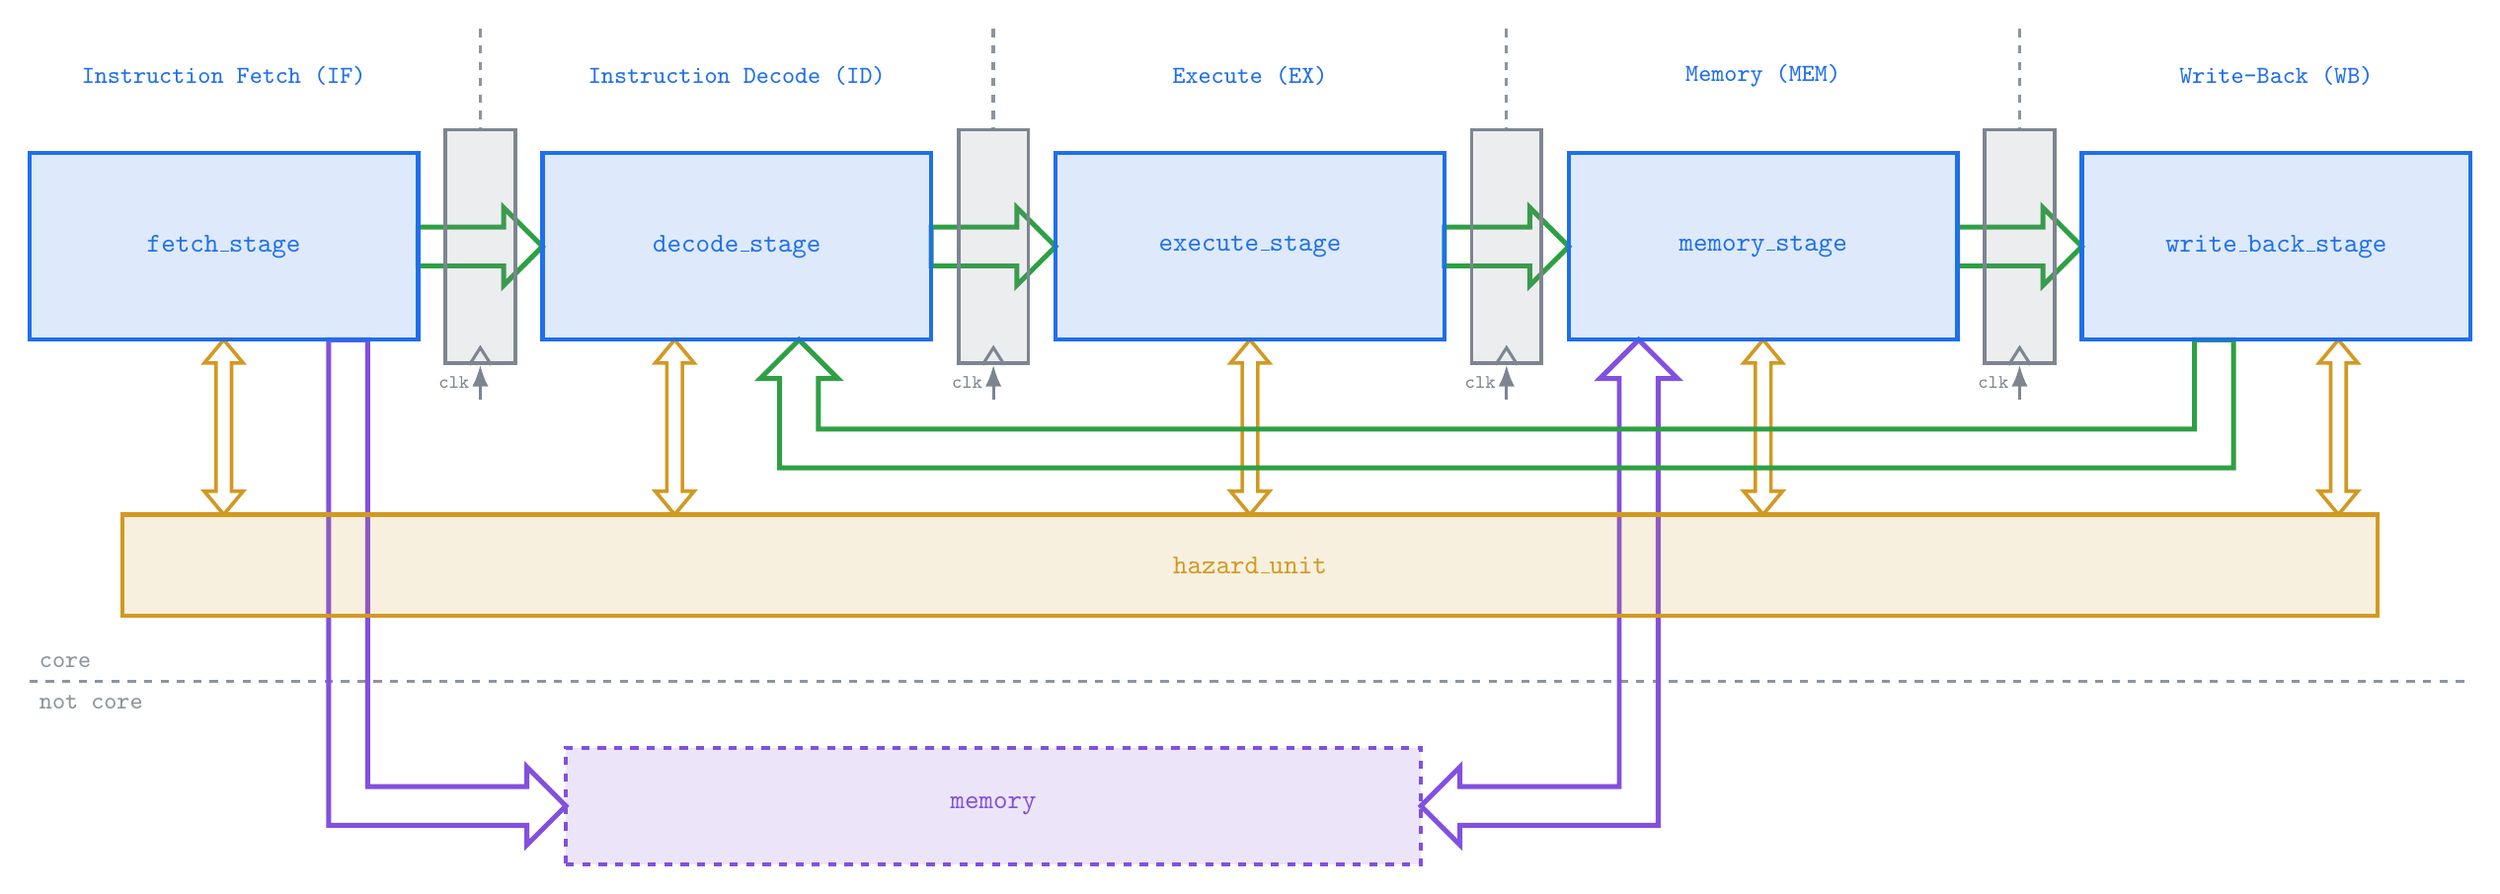
\begin{tikzpicture}[
    >=Latex,
    font=\small,
    % Stage box (15% opaque background, sharp corners, generous text padding)
    stagebox/.style={
        draw=stagecolor, line width=1.5pt,
        fill=stagecolor, fill opacity=0.15, text opacity=1.0,
        minimum width=5.0cm, minimum height=2.4cm, align=center,
        text=stagecolor, font=\bfseries\normalsize,
        inner xsep=14pt, inner ysep=8pt
    },
    % Pipeline register box (15% opaque background, no text, sharp corners)
    pipereg/.style={
        draw=regcolor, line width=1.3pt,
        fill=regcolor, fill opacity=0.15,
        minimum width=0.9cm, minimum height=3.0cm
    },
    % Hazard unit box (15% opaque background, sharp corners)
    hazardbox/.style={
        draw=hazardcolor, line width=1.5pt,
        fill=hazardcolor, fill opacity=0.15, text opacity=1.0,
        minimum width=29.0cm, minimum height=1.3cm, align=center,
        text=hazardcolor, font=\bfseries\normalsize,
        inner xsep=10pt, inner ysep=8pt
    },
    % Dashed memory block (15% opaque background, sharp corners)
    membox/.style={
        draw=arrowpurple, dashed, line width=1.5pt,
        fill=arrowpurple, fill opacity=0.15, text opacity=1.0,
        minimum width=11.0cm, minimum height=1.5cm, align=center,
        text=arrowpurple, font=\bfseries\normalsize,
        inner xsep=14pt, inner ysep=8pt
    },
    stagetitle/.style={
        font=\bfseries\small, text=stagecolor, align=center
    },
    clkline/.style={line width=1.1pt, draw=regcolor},
    stageline/.style={dashed, draw=boundarycolor, line width=1.2pt},
    coreboundary/.style={dashed, draw=boundarycolor, line width=1.2pt}
]

% Coordinate spacing:
% Stages at x = 0, 6.6, 13.2, 19.8, 26.4 (width 5.0cm)
% Pipeline registers at x = 3.3, 9.9, 16.5, 23.1 (width 0.9cm)

% ========================================================
% Full Stage Names Above & Dashed lines above registers
% ========================================================
\node[stagetitle] at (0,    2.2) {Instruction Fetch (IF)};
\node[stagetitle] at (6.6,  2.2) {Instruction Decode (ID)};
\node[stagetitle] at (13.2, 2.2) {Execute (EX)};
\node[stagetitle] at (19.8, 2.2) {Memory (MEM)};
\node[stagetitle] at (26.4, 2.2) {Write-Back (WB)};

\foreach \x in {3.3, 9.9, 16.5, 23.1} {
    \draw[stageline] (\x, 2.8) -- (\x, 1.5);
}

% ========================================================
% Core / Not Core Boundary Line
% ========================================================
\draw[coreboundary] (-2.5, -5.60) -- (28.9, -5.60);
\node[anchor=south west, font=\bfseries\small, text=boundarycolor] at (-2.5, -5.55) {core};
\node[anchor=north west, font=\bfseries\small, text=boundarycolor] at (-2.5, -5.65) {not core};

% ========================================================
% ARROW LAYER 1 (BOTTOM OF ARROWS): Yellow Bi-Directional Arrows
% Stages <-> Hazard Unit
% Shaft thickness 0.20cm, wing width 0.50cm, head length 0.30cm
% Flush with stages at y = -1.20 and hazard unit at y = -3.45
% ========================================================
\newcommand{\bioutlinearrow}[3]{
  \draw[draw=hazardcolor, line width=1.3pt, fill=none]
    (#1, #2) -- ($(#1, #2) + (-0.25, -0.30)$) -- ($(#1, #2) + (-0.10, -0.30)$)
    -- ($(#1, #3) + (-0.10, 0.30)$) -- ($(#1, #3) + (-0.25, 0.30)$)
    -- (#1, #3)
    -- ($(#1, #3) + (0.25, 0.30)$) -- ($(#1, #3) + (0.10, 0.30)$)
    -- ($(#1, #2) + (0.10, -0.30)$) -- ($(#1, #2) + (0.25, -0.30)$)
    -- cycle;
}

\foreach \x in {0, 5.8, 13.2, 19.8, 27.2} {
    \bioutlinearrow{\x}{-1.20}{-3.45}
}

% ========================================================
% ARROW LAYER 2 (MIDDLE OF ARROWS): Purple 90-Degree Arrows (Memory)
% Same thickness as green arrows (shaft 0.50cm, head length 0.50cm, wing span 1.00cm)
% Flush with stage bottoms at y = -1.20 and memory block sides at x = 4.40 / 15.40
% ========================================================
% Fetch stage -> Memory block (instruction fetch): goes bottom then turns toward memory
\draw[draw=arrowpurple, line width=1.8pt, fill=none]
  (1.35, -1.20) -- (1.35, -7.45)
  -- (3.90, -7.45) -- (3.90, -7.70) -- (4.40, -7.20) -- (3.90, -6.70) -- (3.90, -6.95)
  -- (1.85, -6.95) -- (1.85, -1.20) -- cycle;

% Memory stage <-> Memory block (data access): single bi-directional 90-degree arrow
\draw[draw=arrowpurple, line width=1.8pt, fill=none]
  (18.20, -1.20) -- (18.70, -1.70) -- (18.45, -1.70)
  -- (18.45, -7.45) -- (15.90, -7.45) -- (15.90, -7.70) -- (15.40, -7.20) -- (15.90, -6.70) -- (15.90, -6.95)
  -- (17.95, -6.95) -- (17.95, -1.70) -- (17.70, -1.70) -- cycle;

% ========================================================
% ARROW LAYER 3 (TOP OF ARROWS): Green Outlined Arrows
% ========================================================
\newcommand{\fwdoutlinearrow}[2]{
  \draw[draw=arrowgreen, line width=1.8pt, fill=none]
    (#1, 0.25) -- ($(#2, 0.25) + (-0.50, 0)$)
    -- ($(#2, 0.50) + (-0.50, 0)$) -- (#2, 0)
    -- ($(#2, -0.50) + (-0.50, 0)$) -- ($(#2, -0.25) + (-0.50, 0)$)
    -- (#1, -0.25) -- cycle;
}

% Fetch -> Decode (overlapping r1)
\fwdoutlinearrow{2.50}{4.10}

% Decode -> Execute (overlapping r2)
\fwdoutlinearrow{9.10}{10.70}

% Execute -> Memory (overlapping r3)
\fwdoutlinearrow{15.70}{17.30}

% Memory -> Write-Back (overlapping r4)
\fwdoutlinearrow{22.30}{23.90}

% U-Shaped Outlined Arrow: Flush with WB and Decode at y = -1.20
% Shaft thickness 0.50cm (matching forward arrows), arrowhead width 1.00cm
% Horizontal bar at y = -2.35 .. -2.85 for clear clk arrow spacing
\draw[draw=arrowgreen, line width=1.8pt, fill=none]
  (25.35, -1.20) -- (25.35, -2.35)
  -- (7.65, -2.35) -- (7.65, -1.70)
  -- (7.90, -1.70) -- (7.40, -1.20) -- (6.90, -1.70)
  -- (7.15, -1.70) -- (7.15, -2.85)
  -- (25.85, -2.85) -- (25.85, -1.20) -- cycle;

% ========================================================
% BLOCKS LAYER (TOP LEVEL): All blocks drawn on top of arrows
% 50% opaque background matching border colors
% ========================================================
% Per-stage module blocks
\node[stagebox] (fetch)  at (0,    0) {\texttt{fetch\_stage}};
\node[stagebox] (decode) at (6.6,  0) {\texttt{decode\_stage}};
\node[stagebox] (exec)   at (13.2, 0) {\texttt{execute\_stage}};
\node[stagebox] (mem)    at (19.8, 0) {\texttt{memory\_stage}};
\node[stagebox] (wb)     at (26.4, 0) {\texttt{write\_back\_stage}};

% Pipeline Registers between stages
\node[pipereg] (r1) at (3.3,  0) {};
\node[pipereg] (r2) at (9.9,  0) {};
\node[pipereg] (r3) at (16.5, 0) {};
\node[pipereg] (r4) at (23.1, 0) {};

% Hazard Unit
\node[hazardbox] (hazard) at (13.2, -4.1) {\texttt{hazard\_unit}};

% Dashed Memory Block: Under Hazard Unit, below Decode & Execute
\node[membox] (memory) at (9.9, -7.20) {\texttt{memory}};

% ========================================================
% Clocks on registers (drawn on top of registers)
% ========================================================
\foreach \reg in {r1, r2, r3, r4} {
    % Clock triangle symbol on bottom edge of register
    \draw[clkline] ($(\reg.south) + (-0.14, 0)$) -- ($(\reg.south) + (0, 0.22)$) -- ($(\reg.south) + (0.14, 0)$);
    % Clock input line
    \draw[clkline, ->] ($(\reg.south) + (0, -0.45)$) -- node[left, font=\scriptsize\color{regcolor}] {clk} ($(\reg.south) + (0, 0)$);
}

\end{tikzpicture}
\end{document}
